\documentclass[aps,prl,reprint,amsmath,amssymb,superscriptaddress,nofootinbib,floatfix]{revtex4-2}
\usepackage{graphicx}
\usepackage{bm}
\usepackage{mathtools}
\usepackage{microtype}
\usepackage{tikz}
\usetikzlibrary{arrows.meta,positioning,calc,fit}
\usepackage{pgfplots}
\usepgfplotslibrary{groupplots,fillbetween}
\pgfplotsset{compat=1.18}
\definecolor{deepblue}{RGB}{30,76,120}
\definecolor{warmred}{RGB}{170,64,52}
\definecolor{softgray}{RGB}{95,95,95}
\newcommand{\Prb}{\operatorname{Pr}}
\newcommand{\Tr}{\operatorname{Tr}}
\newcommand{\Mmap}{\mathcal{M}}
\newcommand{\Cretro}{C_{\mathrm{retro}}}
\newcommand{\Qretro}{Q_{\mathrm{retro}}}
\newcommand{\Cfwd}{C_{\rightarrow}}
\newcommand{\Qfwd}{Q_{\rightarrow}}
\newcommand{\Imax}{I_{\max}}
\newcommand{\Idoe}{I_{\mathrm{doe}}}
\begin{document}
\title{Phase Transition in Retrocausal Communication}
\author{Z. Hunter}
\affiliation{Independent Researcher, Barcelona, Spain}
\date{July 26, 2026}
\begin{abstract}
Ji, Lloyd, and Wilde recently defined future-to-past communication capacities for a noisy postselected closed timelike curve represented by a completely positive map. We construct a family of such maps from local noisy Bell boundaries on a graph. One boundary has record correlation $d_e=\tanh J_e$; correlations multiply in series, while conditioning a loopy graph produces the Ising correlation $D_{uv}$. The terminal map is binary symmetric, with $\Cretro=2\Qretro=2\operatorname{artanh}(D_{uv})/\ln2$. Hence an Ising ordering transition becomes a transition in retrocausal capacity. The exact square-lattice threshold is $d_c=\sqrt2-1$; for the simple-cubic lattice $d_c=0.218095$. At criticality the retrocausal rates inherit the Ising two-point exponent, while the ordinary forward classical capacity has twice that exponent and the ordinary quantum capacity is zero. Rates are per supplied complete network map; a forward-time heralded realization has an acceptance cost exponential in the network size.
\end{abstract}
\maketitle
\textit{Introduction.---}
Ji, Lloyd, and Wilde (JLW) recently defined classical and quantum capacities for a noisy postselected closed timelike curve (P-CTC) represented by a completely positive (CP) map from a future input to a past output~\cite{Ji2026}. Their theorem characterizes one supplied map. We ask what happens when that map is built from many local consistency bonds. An isolated bond transmits a normalized record correlation $d_e=\tanh J_e$. Along a fixed path the endpoint correlation is the product of the $d_e$ and therefore falls exponentially with length. A graph with cycles contains many compatible edge subgraphs joining the same terminals. The question is whether spatial composition can turn the same analytic local correlation into a nonzero communication rate at macroscopic distance.

Each edge uses the postselected-teleportation boundary introduced for P-CTCs by Lloyd \textit{et al.}~\cite{Lloyd2011}. A loop qubit interacts with two record qubits through a parity-controlled unitary, undergoes a bit-flip channel, and is projected with its reference onto the Bell state used for preparation. Contracting one boundary gives a trace-decreasing parity map. Contracting every edge boundary and discarding the internal records gives one terminal CP map, which serves as the noisy future-to-past resource in the JLW task. A chronology-respecting heralded circuit can reproduce the same trace-decreasing map conditionally, but it does not create a P-CTC. Huang \textit{et al.} recently implemented a circuit of this latter kind for P-CTC decoding of scrambled information~\cite{Huang2026}.

Several established results are close in method but concern different communication tasks. Broadcasting on a noisy tree is an Ising reconstruction problem~\cite{Evans2000}. Plenio and Virmani related many-body criticality to forward channels whose errors are correlated across repeated uses~\cite{Plenio2007,Plenio2008}. Postselected communication conditions the decoding error on a conclusive outcome, without placing the channel from future to past~\cite{JiRegulaWilde2024}. Measurement-conditioned dynamics instead exhibit transitions in entanglement, purification, or information recovery~\cite{Skinner2019,Choi2020,Gullans2020,Roser2026}.

We derive the graph map and its rates exactly. Paths reproduce serial composition, cycles replace the path product by an Ising two-point function, and growing hypercubic lattices inherit the corresponding Ising transition. The square lattice is exact; the simple-cubic lattice gives the locally connected three-dimensional case.

\begin{figure*}[t]
\centering
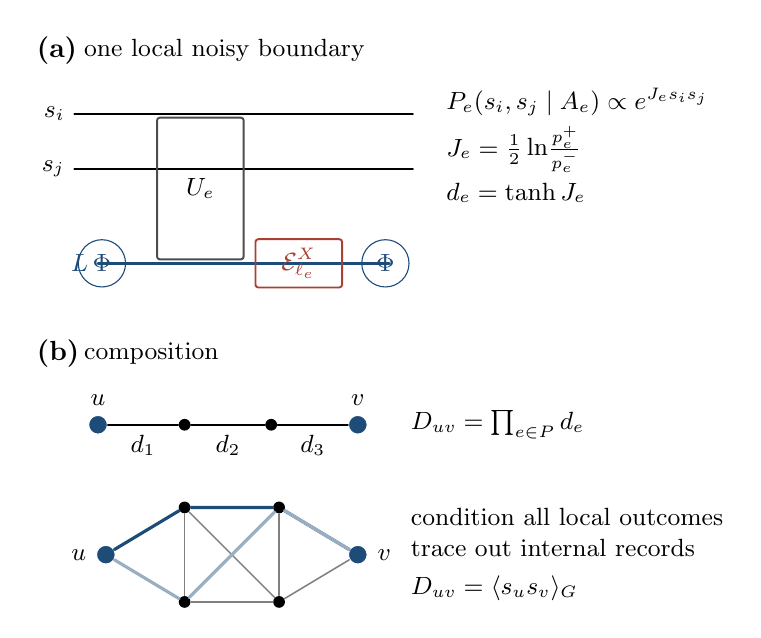
\begin{tikzpicture}[font=\small,>=Latex,line cap=round,line join=round,
record/.style={circle,fill=black,inner sep=1.5pt},
terminal/.style={circle,fill=deepblue,draw=white,line width=.4pt,inner sep=2.4pt},
box/.style={rounded corners=1pt,draw=black!70,line width=.7pt,minimum width=11mm,minimum height=6mm,align=center}]
\node[font=\bfseries,anchor=west] at (-0.2,3.75) {(a)};
\node[anchor=west] at (0.4,3.75) {one local noisy boundary};
\draw[line width=.75pt] (0.4,2.95)--(4.7,2.95);
\draw[line width=.75pt] (0.4,2.25)--(4.7,2.25);
\node[left] at (0.4,2.95) {$s_i$};\node[left] at (0.4,2.25) {$s_j$};
\draw[line width=.9pt,deepblue] (0.7,1.05)--(4.4,1.05);
\node[left,deepblue] at (0.7,1.05) {$L$};
\node[box,minimum height=18mm] (U) at (2.0,2.0) {$U_e$};
\node[box,draw=warmred,text=warmred] (N) at (3.25,1.05) {$\mathcal E^X_{\ell_e}$};
\node[circle,draw=deepblue,text=deepblue,minimum size=6mm,inner sep=0pt] at (0.75,1.05) {$\Phi$};
\node[circle,draw=deepblue,text=deepblue,minimum size=6mm,inner sep=0pt] at (4.35,1.05) {$\Phi$};
\node[align=left,anchor=west] at (5.0,2.55) {$P_e(s_i,s_j\mid A_e)\propto e^{J_es_is_j}$\\[1mm]$J_e=\frac12\ln\!\frac{p_e^+}{p_e^-}$\\[1mm]$d_e=\tanh J_e$};
\node[font=\bfseries,anchor=west] at (-0.2,-0.1) {(b)};
\node[anchor=west] at (0.4,-0.1) {composition};
\node[terminal,label=above:$u$] (pu) at (0.7,-1.0) {};
\node[record] (p1) at (1.8,-1.0) {};\node[record] (p2) at (2.9,-1.0) {};
\node[terminal,label=above:$v$] (pv) at (4.0,-1.0) {};
\draw[line width=.8pt] (pu)--node[below]{$d_1$}(p1)--node[below]{$d_2$}(p2)--node[below]{$d_3$}(pv);
\node[anchor=west] at (4.55,-1.0) {$D_{uv}=\prod_{e\in P}d_e$};
\node[terminal,label=left:$u$] (u) at (0.8,-2.65) {};
\node[record] (a1) at (1.8,-2.05) {};\node[record] (a2) at (3.0,-2.05) {};
\node[record] (b1) at (1.8,-3.25) {};\node[record] (b2) at (3.0,-3.25) {};
\node[terminal,label=right:$v$] (v) at (4.0,-2.65) {};
\foreach \x/\y in {u/a1,a1/a2,a2/v,u/b1,b1/b2,b2/v,a1/b1,a2/b2,a1/b2,b1/a2}{\draw[black!50,line width=.55pt] (\x)--(\y);}
\draw[deepblue,line width=1.15pt] (u)--(a1)--(a2)--(v);
\draw[deepblue!45,line width=1.15pt] (u)--(b1)--(a2)--(v);
\node[align=left,anchor=west] at (4.55,-2.65) {condition all local outcomes\\trace out internal records\\[1mm]$D_{uv}=\langle s_us_v\rangle_G$};
\end{tikzpicture}
\caption{One local bond and its two composition laws. (a) A noisy postselected Bell boundary produces one parity-weighted consistency bond with normalized correlation $d_e=\tanh J_e$. (b) Along a path, correlations multiply. On a graph with cycles, shared internal records make the composition collective: after conditioning the full graph and tracing out the internal records, the endpoint correlation is the Ising two-point function.}
\label{fig:network}
\end{figure*}

\textit{Local boundary and terminal map.---}
Let $G=(V,E)$ be a finite connected graph. Vertex $i$ carries a qubit with computational-basis label $s_i\in\{\pm1\}$. For an edge $e=(ij)$, let $p_e^+$ and $p_e^-$ be the success probabilities of the final Bell projection when $s_is_j=+1$ and $s_is_j=-1$, respectively, with $1\ge p_e^+\ge p_e^->0$. Define
\begin{align}
 J_e&=\frac12\ln\frac{p_e^+}{p_e^-},&
 d_e&:=\tanh J_e=\frac{p_e^+-p_e^-}{p_e^++p_e^-},\nonumber\\
 p_e(s_is_j)&=\sqrt{p_e^+p_e^-}\,e^{J_es_is_j}.
\label{eq:edge}
\end{align}
Retaining the selected Bell outcome gives
\begin{equation}
 \Lambda_e(\rho)=p_e^+\Pi_e^+\rho\Pi_e^+ +p_e^-\Pi_e^-\rho\Pi_e^-,\qquad \Pi_e^\pm=\frac{I\pm Z_iZ_j}{2}.
\label{eq:localmap}
\end{equation}
The Supplemental Material derives Eq.~\eqref{eq:localmap} from the Bell-boundary circuit in Fig.~\ref{fig:network}(a)~\cite{Lloyd2011,SM}. The quantity $d_e$ is the correlation of the normalized one-edge channel. The projectors for different edges are diagonal in the same record basis, so the maps $\Lambda_e$ commute.

Choose distinct terminals $u$ and $v$. The state at $u$ is the input; every other vertex is initialized maximally mixed. After applying all edge maps, discard every system except $v$:
\begin{align}
 \Lambda_G&=\mathop{\circ}_{e\in E}\Lambda_e,\nonumber\\
 \Mmap_{G,u\to v}(\rho_u)&=\Tr_{V\setminus\{v\}}\Lambda_G\!\left(\rho_u\otimes\frac{I_{V\setminus\{u\}}}{2^{|V|-1}}\right).
\label{eq:globalmap}
\end{align}
An edge incident on $u$ removes the input coherences. All other registers start diagonal, and every later parity map preserves diagonality. The output at $v$ is therefore classical in the $Z$ basis.

Let $A$ denote success of every local Bell projection. For fixed endpoint values $s_u=a$ and $s_v=b$, the unnormalized transition weight is
\begin{equation}
 M_G(b|a)=2^{-(|V|-1)}\sum_{\substack{\bm s:\,s_u=a\\s_v=b}}\prod_{e=(ij)}p_e(s_is_j).
\label{eq:terminalM}
\end{equation}
A global spin flip leaves every edge product unchanged, so the column sum $c_G:=\sum_bM_G(b|a)=\Prb(A|s_u=a)$ is independent of $a$. Define the zero-field Ising partition function and terminal two-point correlation
\begin{align}
 Z_G(\bm J)&=\sum_{\bm s}\exp\!\left(\sum_{e=(ij)}J_es_is_j\right),\nonumber\\
 D_{uv}&=\frac{1}{Z_G(\bm J)}\sum_{\bm s}s_us_v\exp\!\left(\sum_{e=(ij)}J_es_is_j\right).
\label{eq:Dcorr}
\end{align}
Spin-flip symmetry gives the two-spin marginal $[1+abD_{uv}]/4$, and therefore
\begin{equation}
 \Mmap_{G,u\to v}(\rho)=c_G\sum_{a,b=\pm1}\frac{1+abD_{uv}}{2}\langle a|\rho|a\rangle |b\rangle\!\langle b|.
\label{eq:map}
\end{equation}
Thus the normalized terminal map is a binary symmetric channel with correlation $D_{uv}$.

On a path, writing $\mathcal B_d(b|a)=(1+abd)/2$,
\begin{equation}
 \mathcal B_{d_{e_n}}\circ\cdots\circ\mathcal B_{d_{e_1}}=\mathcal B_{\prod_kd_{e_k}},\qquad D_{uv}=\prod_{e\in\operatorname{path}(u,v)}d_e.
\label{eq:serialcomposition}
\end{equation}
A graph with cycles is not a serial composition of independent path channels: adjacent edge operations act on shared internal records, and the endpoint map is defined only after the complete conditioned graph operation and the removal of those records. The high-temperature expansion makes the distinction explicit:
\begin{equation}
 D_{uv}=\frac{\displaystyle\sum_{F:\,\partial F=\{u,v\}}\prod_{e\in F}d_e}{\displaystyle\sum_{F:\,\partial F=\varnothing}\prod_{e\in F}d_e}.
\label{eq:strings}
\end{equation}
For a tree, the denominator contains only the empty subgraph and the numerator contains the unique path. The equivalent Fortuin--Kasteleyn connectivity representation is derived in the Supplemental Material~\cite{SM,FortuinKasteleyn1972,EdwardsSokal1988}.

\textit{Capacity as a function of the Ising correlation.---}
For a CP map $\mathcal N$, JLW express the asymptotic rates as $\Cretro(\mathcal N)=2\Qretro(\mathcal N)=\Imax(\mathcal N)+\Idoe^{\infty}(\mathcal N)$~\cite{Ji2026}. Evaluating these quantities for Eq.~\eqref{eq:map} gives
\begin{equation}
 \Cretro(G;u,v)=2\Qretro(G;u,v)=\log_2\frac{1+D_{uv}}{1-D_{uv}}.
\label{eq:capacity}
\end{equation}
Writing $\rho_{uv}:=\operatorname{artanh}D_{uv}$ gives $\Cretro=2\rho_{uv}/\ln2$. For one edge $\rho_{uv}=J_e$; parallel boundaries add $J_e$, while series links multiply $d_e$~\cite{SM}. We call this coordinate rapidity-like only in this algebraic sense.

When the same normalized binary map is used in the ordinary forward-time direction,
\begin{equation}
 \Cfwd(D)=1-h_2\!\left(\frac{1-D}{2}\right),\qquad \Qfwd=0.
\label{eq:forwardC}
\end{equation}
For $D\ll1$,
\begin{equation}
 \Cretro(D)=\frac{2D}{\ln2}+O(D^3),\qquad \Cfwd(D)=\frac{D^2}{2\ln2}+O(D^4).
\label{eq:weakD}
\end{equation}
Thus a critical correlation $D(r)\sim r^{-x}$ gives retrocausal exponent $x$ and forward classical-capacity exponent $2x$.

\textit{Lattice dimension.---}
For a periodic nearest-neighbor hypercubic lattice, let $J_c^{(\mathsf d)}$ be the Ising critical coupling. Then $d_c^{(\mathsf d)}=\tanh J_c^{(\mathsf d)}$. A chain has no finite-$J$ transition. For the square lattice, taking the thermodynamic limit before the long-distance limit gives the spin-flip-symmetric Gibbs state, with ordered-phase $D_\infty=m^2$. The exact threshold is
\begin{equation}
 \Gamma_c=1+\sqrt2,\qquad d_c=\sqrt2-1,\qquad \ell_c=1-\frac1{\sqrt2}.
\label{eq:critical}
\end{equation}
Yang's magnetization gives
\begin{equation}
 D_\infty(d)=\left[1-\left(\frac{1-d^2}{2d}\right)^4\right]^{1/4},\qquad d>d_c.
\label{eq:Dinf}
\end{equation}
At criticality $D(r)\sim r^{-1/4}$, so $\Cretro(r)\sim r^{-1/4}$ and $\Cfwd(r)\sim r^{-1/2}$~\cite{Montroll1963,Wu1976}. For the simple-cubic lattice, $J_c^{(3)}=0.221654626(5)$ gives $d_c^{(3)}=0.21809455$ and $\ell_c^{(3)}=0.39095272$~\cite{Ferrenberg2018}. With $\eta_3=0.0362978(20)$~\cite{Kos2016}, $\Cretro(r)\sim r^{-1.03630}$ and $\Cfwd(r)\sim r^{-2.07260}$.

\begin{figure*}[t]
\centering
\begin{tikzpicture}[font=\small]
\begin{groupplot}[group style={group size=3 by 1,horizontal sep=1.2cm},width=.29\textwidth,height=.205\textheight,tick label style={font=\scriptsize},label style={font=\small},title style={font=\small}]
\nextgroupplot[xlabel={local bond correlation $d$},ylabel={ordered phase},xmin=0,xmax=1,ymin=.4,ymax=3.6,ytick={1,2,3},yticklabels={1D,2D,3D},xtick={0,.2181,.4142,1},xticklabels={$0$,$d_c^{(3)}$,$d_c^{(2)}$,$1$},axis y line*=left]
\addplot[black!20,line width=5pt] coordinates {(0,1)(1,1)};
\addplot[black,line width=5pt] coordinates {(1,1)(1,1)};
\addplot[black!20,line width=5pt] coordinates {(0,2)(.41421356,2)};
\addplot[deepblue,line width=5pt] coordinates {(.41421356,2)(1,2)};
\addplot[black!20,line width=5pt] coordinates {(0,3)(.21809455,3)};
\addplot[warmred,line width=5pt] coordinates {(.21809455,3)(1,3)};
\node[anchor=west] at (axis cs:.48,2.35) {$D_\infty>0$};
\node[anchor=west] at (axis cs:.28,3.35) {$D_\infty>0$};
\nextgroupplot[xlabel={$d$},ylabel={$C_{\mathrm{retro},\infty}$},xmin=.40,xmax=.92,ymin=0,ymax=4.2,samples=220,domain=.4143:.92]
\addplot[deepblue,line width=1.2pt] {ln((1+(1-((1-x^2)/(2*x))^4)^(1/4))/(1-(1-((1-x^2)/(2*x))^4)^(1/4)))/ln(2)};
\draw[densely dashed] (axis cs:.41421356,0)--(axis cs:.41421356,4.2);
\node[anchor=west] at (axis cs:.43,3.5) {exact 2D};
\nextgroupplot[xmode=log,ymode=log,xlabel={distance $r$},ylabel={critical rate},xmin=1,xmax=256,ymin=1e-5,ymax=2]
\addplot[deepblue,line width=1.1pt,domain=1:256,samples=80] {1.1*x^(-.25)};
\addplot[deepblue,dashed,line width=1.1pt,domain=1:256,samples=80] {.45*x^(-.5)};
\addplot[warmred,line width=1.1pt,domain=1:256,samples=80] {.85*x^(-1.0363)};
\addplot[warmred,dashed,line width=1.1pt,domain=1:256,samples=80] {.28*x^(-2.0726)};
\node[deepblue,anchor=west] at (axis cs:2,.95) {2D $C_{\rm retro}$};
\node[deepblue,anchor=west] at (axis cs:2,.18) {2D $C_{\to}$};
\node[warmred,anchor=west] at (axis cs:2,.035) {3D $C_{\rm retro}$};
\node[warmred,anchor=west] at (axis cs:2,.0012) {3D $C_{\to}$};
\end{groupplot}
\end{tikzpicture}
\caption{Dimensional dependence of the communication transition. (a) The same local bond fails to order in one dimension but supports nonzero long-distance correlation above $d_c^{(2)}=\sqrt2-1$ on the square lattice and above $d_c^{(3)}=0.218095$ on the simple-cubic lattice. (b) Exact infinite-distance retrocausal rate for the square lattice. (c) Critical scaling laws in two and three dimensions; solid curves denote retrocausal rates and dashed curves the ordinary forward classical capacity. These are asymptotic guides, not fitted data.}
\label{fig:capacity}
\end{figure*}

\textit{Discussion.---}
The transition is collective: one boundary has $d=\tanh J$, a path has $d^n$, parallel constraints add $J$, and a growing lattice can retain $D_\infty>0$. Equation~\eqref{eq:capacity} converts the terminal correlation directly into rate. The square lattice is exact and the simple-cubic lattice gives the local three-dimensional example; graph dimension need not equal physical dimension.

Equation~\eqref{eq:map} relies on zero-field parity weights, maximally mixed internal records, spin-flip symmetry, and commuting basis filters. Biases or noncommuting filters generally produce a different CP map to which JLW still applies, but not the binary channel or Ising solution used here.

Used forward, the normalized map is entanglement breaking and has zero quantum capacity. The positive $\Qretro$ instead belongs to the JLW future-to-past protocol with its separate noiseless forward memory. The rate is per supplied terminal P-CTC map use, which invokes every edge boundary once. A forward-time simulation must realize the all-edge success event and therefore has exponential raw-trial cost on these lattices. The result characterizes the stipulated P-CTC resource, not ordinary backward signaling.

\begin{thebibliography}{99}
\bibitem{Ji2026} K. Ji, S. Lloyd, and M. M. Wilde, Phys. Rev. Lett. \textbf{136}, 230801 (2026).
\bibitem{JiRegulaWilde2024} K. Ji, B. Regula, and M. M. Wilde, Int. J. Quantum Inf. \textbf{22}, 2440012 (2024).
\bibitem{Lloyd2011} S. Lloyd \textit{et al.}, Phys. Rev. Lett. \textbf{106}, 040403 (2011).
\bibitem{Evans2000} W. Evans, C. Kenyon, Y. Peres, and L. J. Schulman, Ann. Appl. Probab. \textbf{10}, 410 (2000).
\bibitem{Plenio2007} M. B. Plenio and S. Virmani, Phys. Rev. Lett. \textbf{99}, 120504 (2007).
\bibitem{Plenio2008} M. B. Plenio and S. Virmani, New J. Phys. \textbf{10}, 043032 (2008).
\bibitem{Skinner2019} B. Skinner, J. Ruhman, and A. Nahum, Phys. Rev. X \textbf{9}, 031009 (2019).
\bibitem{Choi2020} S. Choi, Y. Bao, X.-L. Qi, and E. Altman, Phys. Rev. Lett. \textbf{125}, 030505 (2020).
\bibitem{Gullans2020} M. J. Gullans and D. A. Huse, Phys. Rev. X \textbf{10}, 041020 (2020).
\bibitem{Roser2026} F. Roser \textit{et al.}, Phys. Rev. Lett. \textbf{136}, 140403 (2026).
\bibitem{Huang2026} Y.-T. Huang \textit{et al.}, Phys. Rev. Research \textbf{8}, 023084 (2026).
\bibitem{SM} See Supplemental Material for derivations and finite-graph checks.
\bibitem{FortuinKasteleyn1972} C. M. Fortuin and P. W. Kasteleyn, Physica \textbf{57}, 536 (1972).
\bibitem{EdwardsSokal1988} R. G. Edwards and A. D. Sokal, Phys. Rev. D \textbf{38}, 2009 (1988).
\bibitem{Montroll1963} E. W. Montroll, R. B. Potts, and J. C. Ward, J. Math. Phys. \textbf{4}, 308 (1963).
\bibitem{Wu1976} T. T. Wu, B. M. McCoy, C. A. Tracy, and E. Barouch, Phys. Rev. B \textbf{13}, 316 (1976).
\bibitem{Ferrenberg2018} A. M. Ferrenberg, J. Xu, and D. P. Landau, Phys. Rev. E \textbf{97}, 043301 (2018).
\bibitem{Kos2016} F. Kos, D. Poland, D. Simmons-Duffin, and A. Vichi, J. High Energy Phys. \textbf{08} (2016) 036.
\end{thebibliography}
\end{document}
